\documentclass{article}
\usepackage{mathtools}
\usepackage{listings}
\usepackage{qtree}
\usepackage{tikz-qtree}

\tikzset{
    labeled/.style = {
        circle, draw, thick, minimum size=1.5em, inner sep=0, label=right:{#1}
    }
}

\begin{document}
\title{CS320 Homework 4}
\author{Dustin Randall}
\maketitle

\section{Give pseudocode for max-heap-delete(A, i) and analyze its time complexity.}
\begin{lstlisting}
MaxHeapDelete(A, i)
    if i < 1 or i > A.length
        throw "Invalid Index"
    A[i] = A[A.Length] // replace with the last element
    A.Length--; // reduce heap size

    if(A[i] > A[Parent(i)])
        IncreaseKey(A, i, A[i])  // O(log n)
    else
        MaxHeapify(A, i) // O(log n)
\end{lstlisting}
To delete a node from a max-heap by index, we replace it with the last node.
The node we replaced could be smaller or larger than the last node, so we need to fix the heap.
If it's larger than its parent, we sift up using IncreaseKey, otherwise we sift down using MaxHeapify.
Both operations take \(O(\log n)\) time, and we'll only use one of them, so the time cost is \(O(\log n)\).

\section{Give an $O(n \cdot log_k)$ time algorithm to merge k sorted lists. Give pseudocode and how it will use mergesort for a k-way sort.}
My idea to merge k sorted lists using a min-heap is to construct a min-heap of size k, where the first element of each list is inserted into the initial array.
The initial array is then heapified, and we know that the minimum element is the root.
We then extract the root element and write it to the output array.
Because we don't want to do another n comparisons, we need to capture some additional context in each element of the heap.
Storing a tuple of (value, list index, element index) allows us to insert the next node without additional comparisons.
The heap then needs to be re-heapified, an operation of \(O(\log k)\) time.
Because each of the n elements is inserted into the heap once, the total time cost is \(O(n \log k)\).
This can be used in a k-way mergesort to reduce the memory cost of merging k lists.
This allows fewer recursive stack frames to be used for merge sort, as each frame divides the remaining lists by k instead of 2.
\begin{lstlisting}
struct Node { 
    int value, listIndex, elementIndex;
    operator < (Node a, Node b) return a.value < b.value
}
MergeLists(Lists, n) 
    Output = new Array[n]
    MinHeap = new MinHeap<Node>(Lists.size + 1)
    for (i = 0 .. Lists.size - 1)
        MinHeap.Insert((Lists[i][0], i, 0))
    for(i = 0 .. n)
        smallest = MinHeap.Pop()
        source = Lists[smallest.listIndex]
        next = smallest.elementIndex + 1
        Output[i] = smallest.value

        if(next < source.size)
            MinHeap.Insert(source[next], smallest.listIndex, next)
    return Output

\end{lstlisting}
\section{Maximize the number of nodes where no node's direct parent is included.}
I start with the observation that the majority of nodes are near the bottom of the tree (there are way more students than professors, more professors than deans, etc.).
We also know that each child has exactly one parent, but each parent may have multiple children.
This suggests that a greedy strategy starting from the bottom and working up will yield the best results.
We can use a post-order traversal of the tree to visit each child node before its parent.
If we include a child node, we need to mark its parent as excluded.
Working up the tree we will in effect include every other row of the tree maximizing the number of included nodes.

\section{Describe the strategy for maximizing the number of tasks scheduled without conflicts.}
We are given a set of tasks which only take 1 unit of time to complete, and can be scheduled after a start time, and must finish before the deadline.
This seems to naturally fit a greedy strategy.
Consider the case [A(1,2), B(0,5), C(0,5), D(0,5), E(0,5)]
The optimal solution is [B, A, C, D, E], which means that simply sorting by either start or end will not find the solution.
Even sorting by the window size (end - start) would not produce the solution.
Instead, we need to find the available set of tasks at each time step, and then select the earliest deadline.
We start by sorting the array by start time, and as the time steps increase, we may move the left and right boundary of the array to only include tasks which can start.
After sorting, the list becomes [B, C, D, E, A] and at time point 0, the available set is [B, C, D, E].
We take B, because it has the earliest deadline of 5 and remove it from the set.
At time point 1, the available set is now [C, D, E, A].
We need to select the task with the earliest deadline, which is A.
Following this strategy, we get the output [B, A, C, D, E].

\section{Create a Huffman Tree for the following characters and frequencies: a:40, b:30, c: 90, d: 20, e: 60, f: 120, g:10, h:5}
\subsection*{Huffman Tree}
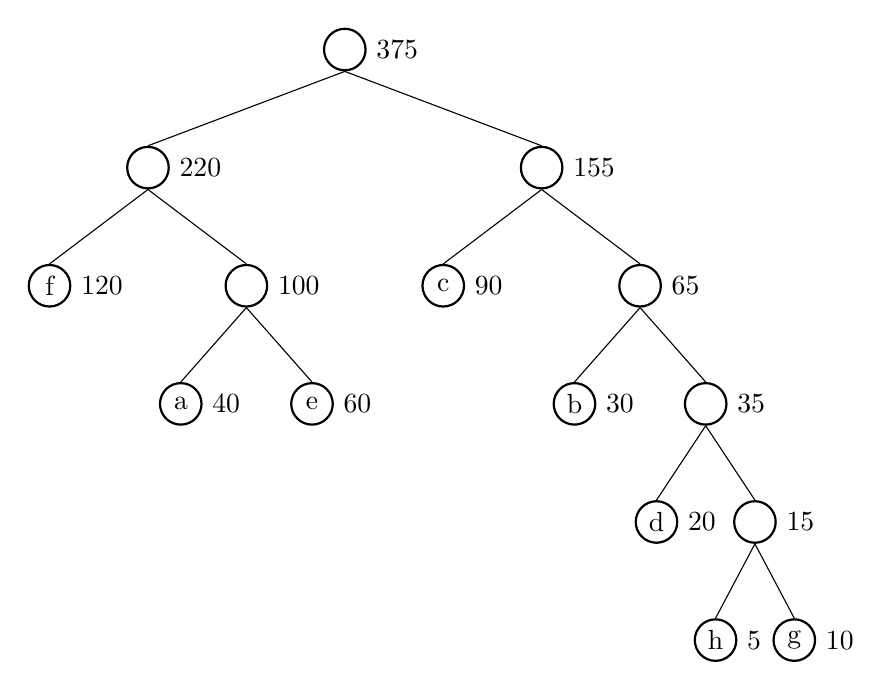
\begin{tikzpicture}[level/.style={sibling distance=50mm/#1}]
    \node[labeled=375]{}
        child {node[labeled=220] {} 
            child {node[labeled=120]{f} }
            child {node[labeled=100]{} 
                child {node[labeled=40]{a} }
                child {node[labeled=60]{e} }
            }
        }
        child {node[labeled=155] {}
            child {node[labeled=90]{c} }
            child {node[labeled=65]{}
                child {node[labeled=30]{b} }
                child {node[labeled=35] {}
                    child {node[labeled=20]{d} }
                    child {node[labeled=15] {}
                        child {node[labeled=5]{h}}
                        child {node[labeled=10]{g}}
                    }
                }
            }
        };

\end{tikzpicture}
\subsection*{Huffman Codes}
\begin{itemize}
    \item a: 010
    \item b: 110
    \item c: 10
    \item d: 1110
    \item e: 011
    \item f: 00
    \item g: 11111
    \item h: 11110
\end{itemize}

\subsection*{Encoded size in bits}
\(40 * 3 + 30 * 3 + 90 * 2 + 20 * 4 + 60 * 3 + 120 * 2 + 10 * 5 + 5 * 5\) \\
\(120 + 90 + 180 + 80 + 180 + 240 + 50 + 25\) \\
\(965\) bits

\subsection*{Compression Ratio}
\(\frac{965}{375 * 8} = \frac{965}{3000} = 0.321\bar{6} = 32.1\bar{6}\%\)

\end{document}